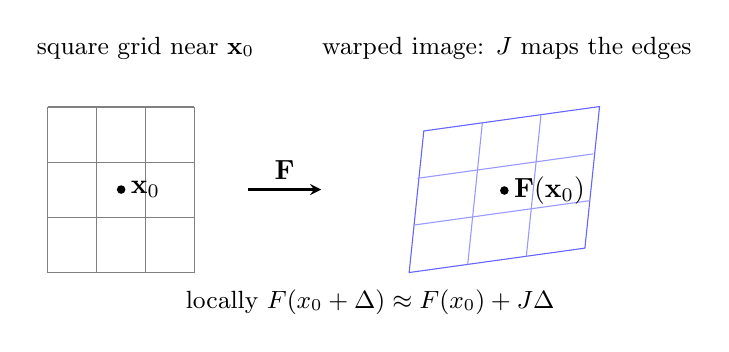
\begin{tikzpicture}[scale=0.62,>=stealth]
\node at (2,4.6) {\small square grid near $\mathbf x_0$};
\foreach \i in {0,1,2,3} \draw[gray] (\i,0)--(\i,3.4);
\foreach \i in {0,1,2,3} \draw[gray] (0,\i*1.13)--(3,\i*1.13);
\fill (1.5,1.7) circle (2.5pt) node[right]{$\mathbf x_0$};
\draw[->,thick] (4.1,1.7)--(5.6,1.7) node[midway,above]{$\mathbf F$};
\begin{scope}[xshift=7.4cm]
\node at (2,4.6) {\small warped image: $J$ maps the edges};
% parallelogram-ish warp
\draw[blue!60] (0,0)--(3.6,0.5)--(3.9,3.4)--(0.3,2.9)--cycle;
\draw[blue!40] (1.2,0.17)--(1.5,3.07);
\draw[blue!40] (2.4,0.33)--(2.7,3.23);
\draw[blue!40] (0.08,0.97)--(3.68,1.47);
\draw[blue!40] (0.17,1.93)--(3.77,2.43);
\fill (1.95,1.68) circle (2.5pt) node[right]{$\mathbf F(\mathbf x_0)$};
\end{scope}
\node at (6.6,-0.6) {\small locally $F(x_0+\Delta)\approx F(x_0)+J\Delta$};
\end{tikzpicture}
